\documentclass[journal]{IEEEtran}
\usepackage{amsmath,amssymb,bm,booktabs,array,multirow,graphicx,cite,url,xcolor,balance}
\usepackage{xurl}
\usepackage[hidelinks]{hyperref}
\hypersetup{pdftitle={Hierarchical RF Tokenization for Parameter-Efficient Cross-Receiver LoRa Fingerprint Identification},pdfauthor={Anonymous working draft},pdfsubject={Frozen-model LoRa mechanism evidence and limited-scope manuscript},pdfkeywords={LoRa, RF fingerprinting, hierarchical tokenization}}
\graphicspath{{figures/}}
\setlength{\tabcolsep}{4pt}
\begin{document}
\title{Hierarchical RF Tokenization for Parameter-Efficient Cross-Receiver LoRa Fingerprint Identification}
\author{Anonymous working draft}
\markboth{Working Research Manuscript, November 22, 2026}{Hierarchical RF Tokenization for Cross-Receiver LoRa Identification}
\maketitle
\begin{abstract}
The process that converts a radio-frequency window into tokens can affect fingerprint identification even when input information, token geometry, and the attention backend are fixed. We study hierarchical RF token formation under a constrained, source-only, closed-set LoRa protocol. A four-stage convolutional tokenizer produces 32 tokens of dimension 64 and is paired with two ordinary multihead-attention blocks. The resulting model has 133,690 parameters. A parameter-matched Patch-Lite control establishes a 2.687 percentage-point accuracy difference on historically developed receivers. Smoothing, support, and normalization controls provide additional, bounded evidence about the design. In a separately frozen external comparison, HStem achieves 97.333\% RX-equal accuracy, compared with 94.208\% for Shen-DANN under native preprocessing; a common in-band control preserves a mean advantage but reveals receiver heterogeneity. Read-only analysis of 24 frozen models finds improved final source-feature separation, while intermediate features challenge a simple receiver-invariance explanation. Complete seed results, GPU costs, and severe synchronization sensitivity are reported. The evidence supports a parameter-efficient system for the present aligned-window protocol, rather than a uniquely identified hardware mechanism or deployment-level authentication guarantee.
\end{abstract}
\begin{IEEEkeywords}
Radio-frequency fingerprint identification, LoRa, cross-receiver identification, tokenization, parameter efficiency, representation analysis.
\end{IEEEkeywords}

\section{Introduction}
\IEEEPARstart{R}{adio-frequency} fingerprint identification (RFFI) uses distinctions in received waveforms to predict transmitter identity. Its security motivation is device-level monitoring, but a received signal also depends on the channel, receiver, acquisition procedure, and preprocessing. A classifier that separates known transmitters at one receiver need not preserve that separation at another. Receiver-aware adversarial training, spectral processing, and information-theoretic regularization address parts of this problem \cite{shen2024receiver,liu2026ask,wang2026ib}. They do not eliminate the need to specify available training data and evaluation scope.

This study asks a narrower architectural question: under fixed in-band RF information and an ordinary attention backend, how does token formation affect identification across receivers? Parameter count alone does not answer this question. A single large patch projection and several local stages can have comparable parameters but different support, normalization, nonlinearities, and optimization behavior. Fewer parameters also need not imply fewer operations or lower latency.

Convolutional token formation and hierarchical processing are established ideas \cite{wu2021cvt,wang2021pvt,liu2021swin}. We do not claim either as a new general principle. Our investigation concerns their controlled use in an existing RF pipeline, where time-domain and frequency-indexed views share a feature-coordinate axis. This construction complicates physical interpretations of local support and shift sensitivity. It motivates experiments that can contradict a mechanism rather than illustrations that presuppose receiver invariance.

We retain strict in-band preprocessing, five RF views, and a shared local front-end from a companion study of receiver-sensitive out-of-band dependence \cite{oobcompanion}. The question and budget differ from that work: the present study replaces token formation and investigates parameter efficiency, support, training parameterization, and their evidence limits. Inherited components, the dataset, and receiver-use history are disclosed rather than counted as new contributions.

Our contributions are threefold.
\begin{enumerate}
\item We develop and evaluate a four-stage RF tokenizer within a fixed 32-by-64 token interface and two-block ordinary MHA classifier. Its contribution is a particular parameter-efficient RF design and controlled empirical behavior, not a new attention operator or the invention of convolutional tokens.
\item We connect parameter-matched and support-related controls to frozen-feature diagnostics. Parameterization, normalization, and layer-wise separation analyses distinguish observations from stronger explanations that remain unproven. Intermediate-layer counterexamples are retained.
\item We provide a source-budget-controlled comparison with Shen CE/DANN, FAN, an IB-RFF adaptation, and the complete LoRa ASKNet implementation. Native and in-band tables, all paired seeds, RX differences, weak fits, and measured GPU costs are jointly reported.
\end{enumerate}

The study is deliberately bounded. Its receivers have a development history, and no new independent acquisition is available. Its inputs are already extracted and aligned. It evaluates closed-set prediction for ten enrolled transmitters, not unknown-device rejection, impersonation resistance, or a complete authentication protocol.

\begin{figure*}[t]
\centering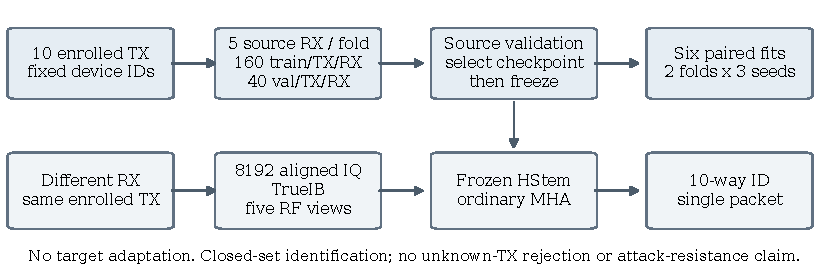
\includegraphics[width=.96\textwidth]{fig01_scope.pdf}
\caption{Task and data flow. A receiver is unseen by a particular trained model, while TX identities remain enrolled. This is not a claim that these RXs were never inspected during the research history. The output is closed-set identity, not an authentication decision with a measured false-acceptance rate.}
\label{fig:scope}
\end{figure*}

\section{Task, Data Permissions, and Prior Work}
\subsection{Closed-Set Cross-Receiver Identification}
Let $y\in\{1,\ldots, 10\}$ identify an enrolled physical transmitter and $r$ denote the receiver. A received window can be described abstractly by
\begin{equation}
 x=\mathcal{R}_{r}\!\left(\mathcal{C}_{h}
       \left(\mathcal{T}_{y}(s)\right)\right)+n ,
\end{equation}
where transmitter, channel, and receiver operators need not be linear or separately identifiable. We learn $f_\theta(x)$ from labeled source-receiver recordings and predict the same transmitter identities at another receiver. Target packets, including unlabeled packets, are not used for adaptation within a fit. RX identities define splits and diagnostics; HStem is trained using TX labels. DANN additionally uses source-RX labels. Figure~\ref{fig:scope} summarizes the permitted data flow.



\subsection{Information Budget and Inherited Components}
The public LoRa receiver corpus \cite{shen2024receiver} supplies fixed 8192-sample complex windows at 1 MHz, SF7, and 125 kHz bandwidth. We retain raw TX labels 31--40, mapped to ten classifier classes. The companion manuscript uses the same broader corpus, including receiver sets used there for development and blind evaluation \cite{oobcompanion}. Its former blind receivers cannot be renamed a newly independent test set.

The inherited TrueIB operator removes out-of-band bins before all downstream views are reconstructed. The five-channel representation and local CNN front-end are also inherited. The present design studies what replaces the large-kernel token projection after that common front-end. Shared inputs, a 32-by-64 token interface, and familiar attention operations are not independent novelty claims.

\subsection{Relation to Cross-Receiver and Tokenization Methods}
Shen et al.\ use channel-independent spectrograms (CIS), receiver-adversarial training, and additional inference or fine-tuning options \cite{shen2024receiver}. We evaluate source-trained, single-packet closed-set variants only; their other options change data or inference permissions. The CE control shares the DANN feature extractor and transmitter head.

FAN and IB-RFF study frequency-aware representations and a two-stage information-bottleneck objective \cite{wang2026ib}. Our 8192-sample adaptation is frozen and labeled; its scores do not reproduce every original dataset or recipe. ASKNet uses learned spectral gating and a unitary Koopman construction \cite{liu2026ask}. We preserve its complete LoRa implementation, including full-dimensional QR, rather than assign WiSig-branch costs to it.

Ma et al.\ combine spectrograms, contrastive pretraining, and Siamese classification \cite{ma2025robust}. This is relevant recent work, but additional pretraining and the original receiver choices require a separately specified adaptation to our permissions. We did not locate an author implementation in the checked paper and author-code sources. It is a coverage limitation; no substitute network or borrowed paper score enters our table.

Convolutional tokens and multistage hierarchies predate this study \cite{wu2021cvt,wang2021pvt,liu2021swin}. Ordinary attention \cite{vaswani2017attention}, BN \cite{ioffe2015batch}, and layer normalization \cite{ba2016layer} are components, not inventions. Shift-stability research \cite{zhang2019shift} motivates diagnostics, but its guarantees cannot be transferred to this RF representation without verification.

\section{Hierarchical RF Token Formation}
\subsection{Signal Preprocessing and Five Views}
For $N=8192$, RMS normalization and the discrete in-band projection are
\begin{align}
 \tilde{x}[n]&=x[n]/\sqrt{N^{-1}\sum_m|x[m]|^2+\epsilon},\\
 x_{\mathrm{IB}}&=\mathcal{F}^{-1}
      \left(M\odot\mathcal{F}(\tilde{x})\right),\quad
 M[k]=\mathbf{1}\{|f_k|\leq 62.5\ {\rm kHz}\}.
\end{align}
The mask retains 1025 bins, including DC and the edge bins. Views are I, Q, standardized log FFT magnitude, log amplitude, and $\operatorname{atan 2}(Q,I)/\pi$. FFT magnitude uses per-window log-domain mean and standard deviation; code preserves the original epsilon and FFT ordering.

The spectral view is indexed by frequency, whereas I/Q and amplitude/phase are indexed by sample position. Concatenating them at the same numerical index is an inherited construction. A receptive field in this shared coordinate system is not a physically isolated RF interval: TrueIB and the FFT view have global dependencies.

\subsection{Shared Front-End and Tokenizer}
The common front-end has stride-one kernel-7 and kernel-5 convolutions, each with 32 channels, BN, and LeakyReLU. HStem applies Table~\ref{tab:arch}; the first three tokenizer stages have BN and GELU and the last is a linear convolution.

\begin{table}[t]\centering
\caption{HStem after the shared 32-channel front-end, initial length 8192.}
\label{tab:arch}
\begin{tabular}{lrrrrr}\toprule
Stage & Kernel & Stride & Pad & Channels & Length\\\midrule
1 & 8 & 4 & 2 & 48 & 2048\\
2 & 8 & 4 & 2 & 64 & 512\\
3 & 8 & 4 & 2 & 64 & 128\\
4 & 4 & 4 & 0 & 64 & 32\\\bottomrule
\end{tabular}
\end{table}

The inherited input projection and learned position terms are followed by pre-normalization, two four-head ordinary MHA blocks, final normalization, mean pooling, and a 64-to-10 linear classifier. Each attention block uses projected Q/K/V, softmax attention, an output projection, and a normalized residual. No new gated mixer or Transformer feed-forward sublayer is introduced. The full model has 133,690 parameters. Figure~\ref{fig:architecture} contrasts the two tokenizers.

\begin{figure*}[t]\centering
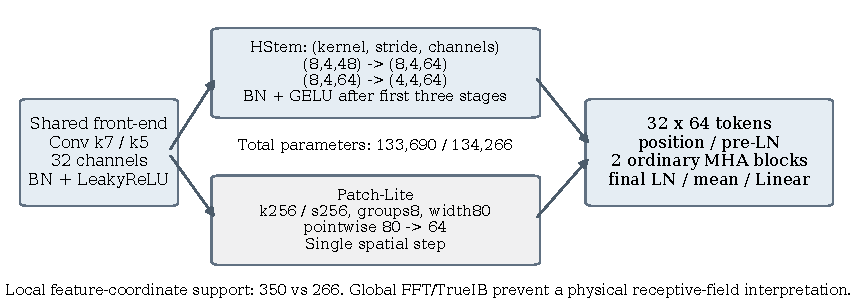
\includegraphics[width=.96\textwidth]{fig02_architecture.pdf}
\caption{Actual architectural comparison. Patch-Lite uses an 80-channel grouped large-kernel projection and a pointwise projection; HStem uses four spatial stages. They share input, front-end, token geometry, and MHA. Parameter matching does not match BN count, nonlinearity, support, or MACs.}
\label{fig:architecture}
\end{figure*}

\subsection{Matched and Mechanism Controls}
Patch-Lite (P0) replaces the tokenizer with a grouped kernel-256/stride-256 projection from 32 to 80 channels (eight groups), followed by a pointwise 80-to-64 projection. A data-free rule selected it within 1\% of full-model parameter count: 134,266, approximately 0.43\% above HStem. The historical full Patch model has 571,434 parameters. HStem versus P0 addresses whether the benefit is solely explained by more parameters, while leaving other differences visible.

H1 expands the learned P0 kernel from 256 to 340 taps by fixed scaled interpolation, retaining stride 256 and padding 42. S1 applies a full-rank 256-to-340-to-256 round trip while retaining the original output support. H2 removes three intermediate tokenizer BN modules; S2 substitutes channel-wise affine transformations, retaining their 352 affine parameters without their statistics.

Including the shared front-end, P0/S1 have local feature-coordinate support 266 and H0/H1/H2/S2 support 350, token stride 256, and first-token center 127.5. H1 and S1 differ in effective frequency response and parameterization as well as support. Removing BN also changes optimization. These controls do not completely isolate a pure hierarchy effect.

\section{Experimental Protocol and Reproducibility}
\subsection{Fixed Packets, Folds, and Selection}
P-H5x 160 samples 200 fixed packets per TX/RX with selection seed 20261012. Of each TX's selected raw rows, the first 160 train and the last 40 validate. Five source RXs give 8000 training and 2000 source-validation packets per fit. Five held RXs give 10,000 evaluation packets without adaptation.

Fold 0 sources are B210-1, RTL-1, RTL-3, RTL-6, RTL-9; held RXs are B200-mini-1, Pluto-1, RTL-2, RTL-5, RTL-7. Fold 1 reverses the sets. Seeds 201/202/203 give six paired fits per complete arm/view. A held receiver in one fold is a source in the other; this does not create twenty independent receivers.

HStem/control training runs 200 epochs, batch 64, CE, and AdamW \cite{loshchilov2019adamw}, learning rate $10^{-3}$, weight decay $5\times 10^{-4}$. Five warmup epochs precede cosine decay. Source training adds AWGN with nominal SNR between 0 and 50 dB; clean source validation selects minimum RX-equal CE. Matched fits share hashed data seeds, permutations, and noise streams. No held-RX score enters a fit's scheduler or selection.

\subsection{External Methods and Information Views}
External paths are CE, DANN, FAN stage 1, IB stage 2, and ASKNet. CE/DANN share encoder/transmitter initialization and noise streams. The TensorFlow-to-PyTorch port passed 103 forward/gradient checks. A misaligned RX validation-label slice in the author entrypoint is repaired and disclosed. Both controls select by source TX CE; DANN's RX loss participates in training. Batch 64, SGD $10^{-3}$, momentum .9, 500-epoch limit, and registered plateau/early-stop rules are retained. Fixed validation noise replaces dynamically resampled noise.

FAN/IB retain two-stage training, Adam $10^{-3}$, batch 128, 200-epoch limits, and source-validation early stopping. Stage 2 starts from its matching stage-1 checkpoint. The 8192 adaptation uses patch 512/stride 256, 31 tokens of width 128, and the original CPU normalized-HSIC computation. Coefficient .004 was fixed from a historically explored adaptation, not optimized on new target scores. Stage 1 is reused for the FAN control rather than trained twice.

ASKNet retains its complete 8191-mode complex transformation, gating candidates 128--4096, batch 128, Adam $10^{-3}$, 200-epoch limit, and patience 20. All seeds are retained. Full-model feasibility and a batch 128 update were checked before fitting. Completed work is 48 CE/DANN/FAN/IB fits and six Native ASK fits, plus six reused HStem checkpoints.

\emph{Native} retains each method's native preprocessing under the same raw-packet permission; HStem keeps its own in-band front-end. \emph{Strict-IB} projects to a common band before the method's frontend. These answer different questions, without asserting equal optimizers or representations. Six ASK Strict-IB fits were deferred as a whole for a recorded compute-budget reason before new Dev inference. They remain unrun/NA.

\subsection{Metrics and Conditional Uncertainty}
Accuracy and macro-F1 are computed per RX, then equally weighted over RXs and seeds. Worst-RX accuracy is the minimum per-RX seed mean. Fit SD is over six fold/seed means and includes fold differences; it is not a standard error over six independent devices.

For paired contrasts, the three seed differences are averaged at each of ten unique RXs, then RX identities are bootstrapped 10,000 times with seed 24016. These conditional intervals omit fresh-seed, acquisition, and architecture-selection uncertainty. All contrasts are reported without multiplicity correction or confirmatory $p$-value claims.

Checkpoint/configuration cohorts were committed and hashed before report-only Dev inference. Baseline/HStem inference used CPU FP32 networks with original frontend precision preserved. ASK used GPU FP32 after six checkpoints were sealed. HStem's new CPU value 97.333\% and historical GPU value 97.335\% are separately retained. Common GPU cost measurement is a separate protocol.

\section{Structural Effects and Representation Evidence}
\subsection{What the Controls Establish}
Table~\ref{tab:ablations} gives matched historical GPU results. HStem exceeds P0 by 2.687\,pp with six positive paired means. This supports the complete tokenizer design at comparable parameters, rather than a pure hierarchy-effect decomposition.

\begin{table}[t]\centering
\caption{Archived matched GPU Dev results, not new S25 training.}
\label{tab:ablations}
\begin{tabular}{lrrrr}\toprule
Arm & Parameters & Support & Acc.(\%) & F1(\%)\\\midrule
P0 Patch-Lite &134266&266&94.648&94.625\\
S1 Round-trip &134266&266&95.527&95.500\\
H1 Expanded &134266&350&96.345&96.321\\
H2 No-mid-BN &133338&350&96.145&96.135\\
S2 Affine-only &133690&350&96.417&96.402\\
H0 HStem &133690&350&97.335&97.326\\\bottomrule
\end{tabular}
\end{table}

\begin{table}[t]\centering
\caption{All four S22 primary contrasts, conditional RX 95\% intervals in pp. The fixed practical rule includes a 0.5\,pp effect and paired/fold consistency; not meeting it does not establish no effect.}
\label{tab:contrasts}
\begin{tabular}{lrrrl}\toprule
Contrast&Mean&95\% interval&Positive&Criterion\\\midrule
H1--S1&.818&[.562, 1.053]&6/6&Pass\\
S1--P0&.878&[.547, 1.252]&5/6&Pass\\
H0--S2&.918&[.492, 1.295]&4/6&Not met\\
S2--H2&.272&[.135,.410]&5/6&Not met\\\bottomrule
\end{tabular}
\end{table}

S1 improves P0 without expanding support; H1 adds an increment beyond S1. Their differences add algebraically to H1--P0, not as independently identified causal mechanisms. H0--H2 is 1.190\,pp, while restoring affine parameters recovers only .272\,pp on average. H0--S2 fails its registered stability condition. These implicate the normalization/training design without proving removal of RX information.

\subsection{Frozen Feature Geometry}
After the external comparison, a no-fit source analysis was registered; a separately committed extension added S1/H1 before their extraction. Historical geometry CSVs contain Dev/Confirm class-distance correlations, not the common source-layer scatter studied here. Existing errors/margins are reused; missing source features alone are extracted.

All 24 H0/P0/S1/H1 models use the same 2000 source-validation packets per fold, noise-free inference, and frozen BN. Mean-pooled tokenizer and pre-MHA outputs and final classifier-input features have dimension 64 and are per-packet L2-normalized. Every tap and paired seed is retained (Fig.~\ref{fig:geometry}).

For normalized $z_{tri}$, define global, TX, and TX-by-RX centroids $\mu,\mu_t,\mu_{tr}$. With $T=10,R=5,n=40$,
\begin{align}
 B_{\rm TX}&=T^{-1}\sum_t\|\mu_t-\mu\|^2,\\
 D_{\rm RX|TX}&=(TR)^{-1}\sum_{t,r}\|\mu_{tr}-\mu_t\|^2,\\
 W&=(TRn)^{-1}\sum_{t,r,i}\|z_{tri}-\mu_{tr}\|^2.
\end{align}
Total balanced scatter equals $B_{\rm TX}+D_{\rm RX|TX}+W$. We report
\begin{equation}
 J_c=\frac{B_{\rm TX}}{D_{\rm RX|TX}+10^{-12}},\quad
 J_w=\frac{B_{\rm TX}}{D_{\rm RX|TX}+W+10^{-12}}.
\end{equation}
At fixed group counts, $J_c$ is proportional to the ratio of between-TX centroid distance to same-TX cross-RX centroid distance. It is a geometric statistic, not mutual information; finite-cell estimation also contributes to $D_{\rm RX|TX}$.

\begin{table*}[t]\centering
\caption{New source-validation diagnostics, already exposed during checkpoint selection. Means are over six fits; ratios are averaged per fit. They are not held-RX generalization results.}
\label{tab:source}\begin{tabular}{lrrrrr}
\toprule Arm & Source Acc. & $B_{\rm TX}$ & $D_{\rm RX|TX}$ & $J_c$ & $J_w$\\ \midrule
P0 & 95.917 & 0.785 & 0.0286 & 27.585 & 4.270 \\
S1 & 96.625 & 0.778 & 0.0281 & 27.818 & 4.435 \\
H1 & 97.467 & 0.805 & 0.0262 & 31.225 & 4.925 \\
H0 & 98.175 & 0.817 & 0.0235 & 35.577 & 5.449 \\
\bottomrule\end{tabular}

\end{table*}
\begin{figure*}[t]\centering
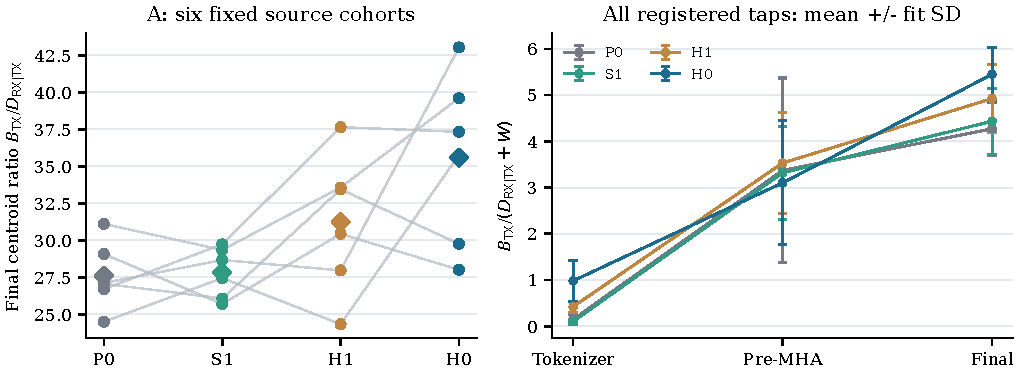
\includegraphics[width=.96\textwidth]{fig03_mechanism_A.pdf}
\caption{Mechanism A. Final centroid ratios for all paired fits (left) and all registered layer taps (right). Pre-MHA means do not have the final ordering. Source validation was already used for selection, so these are descriptive observations.}
\label{fig:geometry}
\end{figure*}

Final mean $J_w$ is 4.270/4.435/4.925/5.449 for P0/S1/H1/H0; H0--P0 is positive in all six pairs. Final $J_c$ is 27.585/27.818/31.225/35.577, with five positive H0--P0 pairs. These support improved final source discrimination in the trained system.

They do not establish direct RX suppression by the tokenizer. Its output has conditional RX scatter .003004 for H0 versus .000185 for P0, higher in every pair. Pre-MHA mean $J_c$ is 33.983 for H0 versus 41.241 for P0. A pooled summary also omits information in the full token sequence. The evidence concerns joint tokenizer/attention training rather than monotone removal of RX content. Supplementary PCA uses all six cohorts and separate, fixed top-two components per model; two-dimensional appearance is not substituted for quantitative evidence.

\subsection{Kernel Evidence and Its Limits}
Existing S23 effective-kernel spectra are reused. High-frequency energy over 0.25--0.5 cycles per frontend position averages 21.808/7.692/4.043\% for P0/S1/H1. Across the 18-model descriptive join, energy has Spearman correlation $-.556$ with final $J_w$ and $+.410$ with final conditional RX scatter. Arm, cohort, parameterization, and optimization confound the association (Fig.~\ref{fig:kernels}).

\begin{figure*}[t]\centering
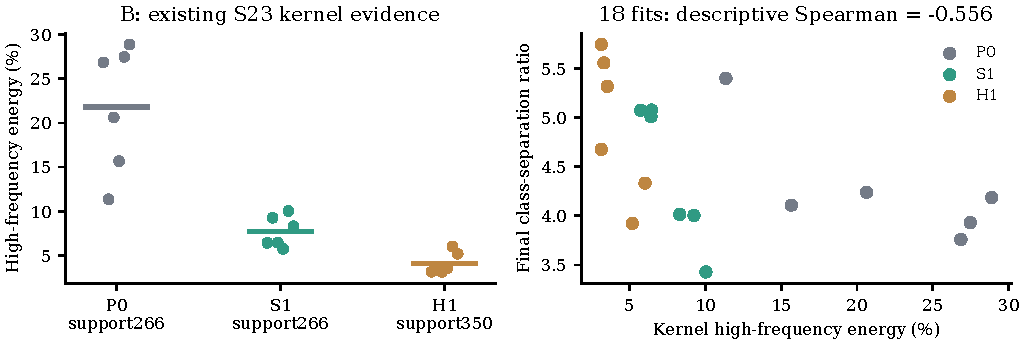
\includegraphics[width=.96\textwidth]{fig04_mechanism_B.pdf}
\caption{Mechanism B. Existing effective-kernel spectra and support (left) joined to new frozen source features (right). These filters act on frontend coordinates, not physical transmitter spectra. All 18 applicable fits are retained.}
\label{fig:kernels}
\end{figure*}

S23 materialized six S1 models as ordinary 256-tap convolutions with bit-identical logits on 12,000 source predictions. For effective kernel $v=Tw$, $T$ has rank 256: the inference function class need not shrink, while optimization coordinates change. A $TT^\top$ interpretation for idealized SGD is not the exact update of AdamW.

Frozen BN can be absorbed into preceding convolutions, but numerical execution matters. Default TF32-enabled execution failed the fixed logit tolerance in all six H0 checks (maximum difference about .01957), although classifications agreed. Disabling TF32 passed the same $10^{-4}$ tolerance (maximum $5.39\times 10^{-5}$). These failures distinguish training effects from removable inference structure.

\subsection{Source Metadata Diagnostics}
Only selected legal source-validation rows of supplied CFO/SNR fields were read. That loader does not read the waveform dataset, the fields never enter a network, and no target CFO/SNR was opened. Raw Spearman correlations with true-class margin are accompanied by fixed TX-by-RX-cell centering; constant residuals are NA.

Across 24 models, raw SNR--margin correlations are negative, but centered correlations range approximately $-.028$ to $.058$. Centered absolute-CFO correlations range approximately $-.057$ to $.032$. This does not establish absence of RF effects: metadata, identity, acquisition, and margin scale are intertwined. It illustrates why raw associations cannot explain held-RX errors. Raw and cosine-weight margins include misclassified samples and every fit.

\section{External Results, RX Heterogeneity, and Cost}
\subsection{Native and Common In-Band Comparison}
\begin{table*}[t]\centering
\caption{Complete S24 comparison on historically developed RXs. Accuracy/F1 are percentages; accuracy is mean $\pm$ fit SD over six fits. Worst is the minimum RX seed-mean accuracy. Strict-IB ASK is deferred, not zero or failed. HStem is the new CPU inference of frozen weights.}
\label{tab:external}\begin{tabular}{lrrrrrr}
\toprule Method & Native Acc. & Strict-IB Acc. & Native F1 & Strict F1 & Native Worst & Strict Worst\\ \midrule
HStem & 97.333 $\pm$ 0.551 & 97.333 $\pm$ 0.551 & 97.325 & 97.325 & 93.683 & 93.683 \\
Shen CE & 93.535 $\pm$ 1.011 & 94.702 $\pm$ 3.111 & 93.347 & 94.283 & 85.817 & 72.150 \\
Shen DANN & 94.208 $\pm$ 1.028 & 94.632 $\pm$ 3.064 & 94.047 & 94.258 & 88.417 & 72.900 \\
FAN & 72.555 $\pm$ 2.683 & 75.827 $\pm$ 2.351 & 71.309 & 75.136 & 62.250 & 71.783 \\
IB-RFF & 73.533 $\pm$ 2.873 & 79.810 $\pm$ 2.731 & 72.427 & 79.291 & 63.450 & 75.683 \\
ASKNet & 65.092 $\pm$ 31.936 & Deferred & 62.995 & -- & 58.900 & -- \\
\bottomrule\end{tabular}

\end{table*}

Table~\ref{tab:external} shows that HStem exceeds the strongest Native mean, Shen-DANN, by 3.125\,pp, conditional interval $[1.075, 5.103]$, with six positive means. Strict-IB's highest competing mean is CE; the difference is 2.632\,pp, interval $[.287, 6.942]$, with five positive means. This is within-protocol competition, not universal state of the art.

DANN--CE is $+.673$pp Native, interval $[.208, 1.233]$, but $-.070$pp Strict-IB, interval $[-.247,.152]$. Adversarial training does not give an additional gain in both settings. IB stage 2 exceeds reused FAN stage 1 by .978\,pp Native (interval $[-.037, 2.195]$) and 3.983\,pp Strict-IB ($[3.373, 4.582]$). These describe the frozen adaptation rather than the general capability of the original method.

\subsection{RX-by-TX Error Attribution}
Mechanism C uses saved S24 predictions and archived error CSVs, not new Dev inference. Native H0--DANN is negative on B200-mini-1 and B210-1 by 2.017 and 1.217\,pp and approximately tied on RTL-6. Means alone conceal these counterexamples; Fig.~\ref{fig:rx} retains all ten RXs.

\begin{figure*}[t]\centering
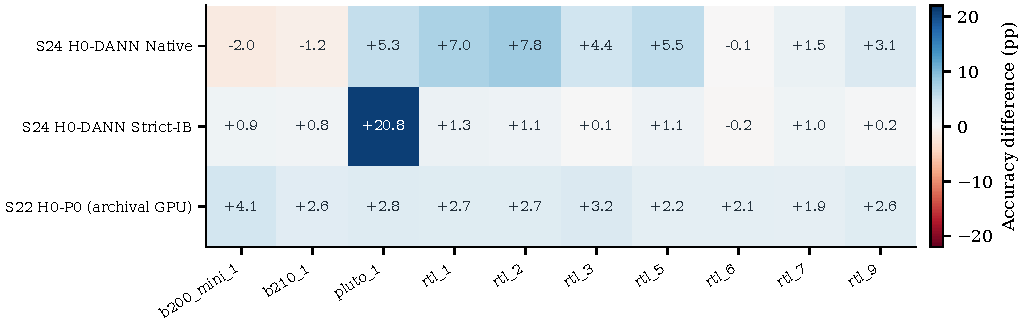
\includegraphics[width=.97\textwidth]{fig05_mechanism_C.pdf}
\caption{Mechanism C: all ten RXs. S24 H0--DANN uses the common new evaluation; H0--P0 is explicitly the matched archival GPU cohort. Positive favors H0. Neither is a newly independent test.}
\label{fig:rx}
\end{figure*}

Strict-IB H0--CE on Pluto-1 is 21.533\,pp: 93.683\% versus 72.150\%. This RX contributes about 82\% of the overall 2.632\,pp difference. The other nine-RX mean difference is .531\,pp; RTL-6 slightly favors CE. This is a post-hoc decomposition, without removing Pluto-1 or changing the primary table.

The common projection improves CE on most other RXs but decreases Pluto-1 from 85.817\% Native to 72.150\% Strict-IB. Its TX32/34/35/39 recalls are 53.833/34.500/10.833/24.333\%, versus H0's 94.500/79.167/82.500/88.333\%. The largest CE confusions are TX35-to-32, TX39-to-38, TX34-to-33, and TX32-to-31. The complete ten-class plot is supplied; these patterns do not uniquely identify CFO, SNR, or RX hardware as a cause.

\subsection{ASK: Retained Weak Fits}
Six Native ASK Dev accuracies are 87.220, 40.670, 74.520, 87.130, 89.320, 11.690\% (mean 65.092\%, fit SD 31.936\,pp). Source accuracies are 90.650, 40.050, 77.350, 90.550, 91.250, 11.500\%. The last selects epoch 1 and stops at 21 under its registered patience 20.

Weak source learning substantially lowers the mean; it does not show that all successful models specifically fail at new receivers. No seed is discarded or replaced. Selecting successful fits would not define a legitimate formal average. Conditional RX intervals do not summarize this seed instability. Stable Shen comparisons carry the main competition argument.

\subsection{Parameter Efficiency Is Not Uniform Speed}
\begin{table*}[t]\centering
\caption{S24 Native GPU-resident IQ-to-logits costs, RTX 4060 Laptop, FP32 networks/TF32 off, original frontend precision retained. Three warmups and 15 samples. B128 is whole-batch time; host transfer is excluded.}
\label{tab:costs}\begin{tabular}{lrrr}
\toprule Method & Parameters & B1 p50 (ms) & B128 p50 (ms)\\ \midrule
HStem & 133,690 & 2.142 & 15.956 \\
Shen CE & 13,442,954 & 1.170 & 22.853 \\
Shen DANN & 13,509,263 & 1.108 & 22.961 \\
FAN & 310,481 & 1.405 & 1.706 \\
IB-RFF & 310,481 & 1.372 & 1.661 \\
ASKNet & 74,153,872 & 2229.082 & 2260.086 \\
\bottomrule\end{tabular}

\end{table*}
\begin{figure*}[t]\centering
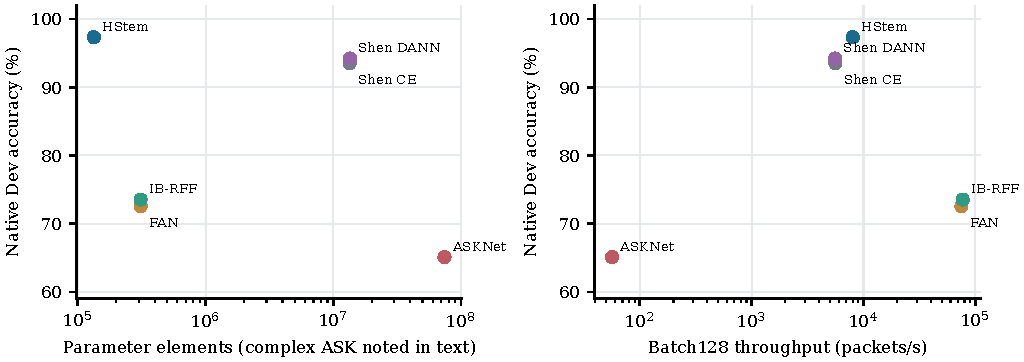
\includegraphics[width=.96\textwidth]{fig06_costs.pdf}
\caption{Accuracy versus parameters and throughput. ASK's 74,153,872 complex/real parameter elements correspond to 141,246,353 real degrees of freedom. Parameter count, latency, and throughput are different axes.}
\label{fig:costs}
\end{figure*}

Table~\ref{tab:costs} and Fig.~\ref{fig:costs} distinguish the cost axes. HStem has approximately one hundredth Shen-DANN's parameter elements. Its batch 128 time is lower, 15.956 versus 22.961\,ms, but batch 1 is higher, 2.142 versus 1.108\,ms. FAN/IB are faster than HStem. A separate new paired H0/P0 session gives 1.866/1.724\,ms batch 1 and 15.164/13.119\,ms batch 128: matched-Patch accuracy gains have a real compute cost.

Literal LoRa ASK takes about 2229\,ms batch 1 and 2260\,ms batch 128, retaining full-dimensional complex QR. This is an implementation measurement, not a reduced-rank or WiSig cost. Dispatcher MACs omit FFT, QR, and unsupported work; they are partial, not complete FLOPs. Separate timing sessions are not pooled, since desktop GPU load and clocks vary.

\section{Failure Boundaries and Innovation Limits}
\subsection{Synchronization Sensitivity}
Frozen source H0 falls from 98.175\% aligned accuracy to 21.858/17.775\% for circular shifts $-4/+4$. P0 also falls to 22.567/16.983\%. Circular shifts preserve contents and Fourier magnitude but are not every physical acquisition error. Locking FFT magnitude to the original barely changes the H0 result (Fig.~\ref{fig:limits}).

\begin{figure*}[t]\centering
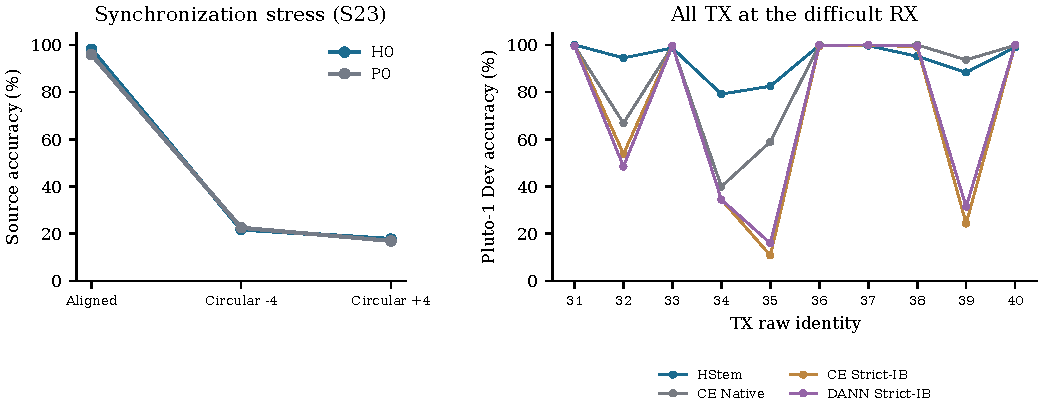
\includegraphics[width=.96\textwidth]{fig07_limits.pdf}
\caption{Negative evidence. Left: archived source-only circular-shift stress, not a target test. Right: every TX on Pluto-1 in saved S24 predictions. Severe shift failure and class-dependent errors remain visible.}
\label{fig:limits}
\end{figure*}

Thus zero padding and magnitude roundoff alone do not explain failure, which is not unique to HStem. Time-domain phase and mixed time/frequency coordinates remain possibilities, not identified causes. Real detection offsets, neighboring continuous samples, and calibrated synchronization distributions are unavailable. Claims are restricted to these pre-extracted aligned windows; synchronization robustness and antialiasing guarantees are unestablished.

\subsection{An Unfitted Long-Patch Audit}
H1--S1 already provides support-related evidence, with its confounds disclosed. We further audited freely learned kernel 340/stride 256/padding 42 candidates without fitting or RF data. They match 350 local support, 32-token geometry, and center 127.5.

Keeping P0's groups 8/width 80 gives 161,146 parameters, about 20.5\% more than H0, and two total BN modules versus five. In a fixed groups/width grid, the within-1\% parameter match has width 8, a rank-at-most-8 linear bottleneck. This threshold does not imply that useful controls are infeasible: groups 8/width 64 gives 138,346 parameters, only 3.48\% more, with a rank-64-capable output. Groups 16/width 112 is 2.32\% below H0 but changes grouping.

The groups 8/width 64 candidate is a feasible optional single-arm, six-fit developmental control. It changes internal width relative to P0 and retains two BN modules versus H0's five, so its outcome would not isolate hierarchy alone. No fit is launched here. Any later execution needs its own frozen design and data permissions; model choice has not used candidate accuracy.

\subsection{Independence and Security Scope}
No new acquisition is available. Current source, Dev, and historical Confirm RXs have development use; the companion used the old six-RX blind set. Existing Location filenames or download timestamps do not prove new independence.

Reusing present classifiers at a new RX also requires the same enrolled physical TXs, known sampling/alignment provenance, and a fresh frozen protocol. Ten different transmitters cannot simply be relabeled 1--10 as the same closed-set test. No independent validation is reported without qualifying data.

Unknown-emitter rejection, false-acceptance/rejection operating points, active imitation, and attacker-controlled synchronization are untested. Closed-set accuracy supports an identification study with security relevance, not a complete authentication guarantee.

\section{Conclusion}
Token formation affects this LoRa cross-RX system beyond nominal parameter count. HStem improves on a matched Patch-Lite control and is competitive in complete external comparisons. Support, parameterization, and normalization experiments narrow possible explanations. New frozen-source diagnostics support final discrimination while retaining counterexamples to simple invariance narratives.

The supported contribution is parameter-efficient RF token construction with controlled evidence. It is not a uniquely identified hardware mechanism, universally faster implementation, new independent test, or synchronization-robust authenticator. Artifacts retain failed criteria, unfavorable RXs, weak seeds, and negative stress tests. More specific mechanism identification and independent acquisition remain open.

\appendices
\section{Artifact and Evidence Map}
Repository: \href{https://github.com/hanCChan/crossatten}{\texttt{hanCChan/crossatten}}. S24 is pinned at \texttt{dde0ef9}; S25 is \texttt{exp/s25-tifs-integration}. Existing checkpoints and protocols are read-only; S25 performs no neural fitting.

The analysis registration freezes source rows, code, evidence, checkpoint hashes, and statistics before new extraction. A separate committed extension records the later S1/H1 and source-metadata request. Initial H0/P0 outputs remain unchanged. This is explicitly exploratory: historical target scores and source selection information were already exposed.

PyTorch \texttt{2.5.0+cu124}, NumPy 1.26.4, and RTX 4060 Laptop hardware are recorded, with exact environment/hashes. Fold-role checks precede IO; packet identities and source cache hashes are checked. Source features use only the original 40 held source packets per TX/RX. CFO/SNR are diagnostics, not inputs. No new Dev, Confirm, or old-blind waveform is loaded.

New-source accuracy agrees with archived selection metrics for 22 of 24 models. P0 fold 0/seed 202 has one fewer correct prediction out of 2000, and S1 fold 0/seed 203 has one more. Checkpoint hashes are unchanged. These small execution differences are disclosed rather than treated as bit-exact recovery; their numerical cause has not been uniquely established. Geometry uses the single frozen analysis execution, while archived stress and target results retain their original values.

S15 supplies parameter matching; S21--S22 supply controls, conditional intervals, rules, errors/margins; S23 supplies kernels, equivalence, and shift failures; S24 supplies external comparisons, a 600,000-prediction audit, and costs. S25 adds 48,000 source predictions from 24 frozen models, all-layer geometry, metadata associations, full RX/TX attribution, and an unfitted architecture audit. Historical evidence is not renamed a new independent repetition.

Large waveforms, checkpoints, and sample-level features remain local. Aggregate tables, registrations, generation code, and the compiled draft are provided. PCA includes every cohort, not a visually selected subset. The missing independent-data experiment is marked not run.

\section{Companion Overlap}
TrueIB, five views, kernel 7/kernel 5 front-end, token geometry, and data origin are inherited \cite{oobcompanion}. The earlier question concerns frozen OOB-pathway dependence with OOB fusion and different mixers/budgets. Here ordinary MHA is held fixed in tokenizer controls. Cross-paper accuracy subtraction would mix several factors and is not architectural causal evidence.

Source-PDF and overlap-audit hashes are retained. The accompanying claim--definition--experiment--result--limitation matrix and ten reviewer questions separate system effects from unproven causal and independence claims. Authorship/affiliations and submission decisions remain to be confirmed outside this anonymous internal consolidation.
\balance
\bibliographystyle{IEEEtran}
\bibliography{references}
\end{document}
